\section{Cronograma}

	Para uma maior organização de esforço e tempo da equipe foi criado um cronograma que fornece uma visão geral e contínua de todo o desenvolvimento do projeto.  O cronograma contempla as fases de Iniciação relacionada com a entrega T1, e fase de Desenvolvimento, incluindo a Sprint 0, e as Releases 1 e 2. Cada fase possui suas respectivas atividades com suas datas de início e fim, tempo de duração e data de conclusão e responsáveis. O conjunto de informações presentes no cronograma tem papel fundamental no controle da execução de todo o processo e numa possível alteração no decorrer dotrabalho.
 
	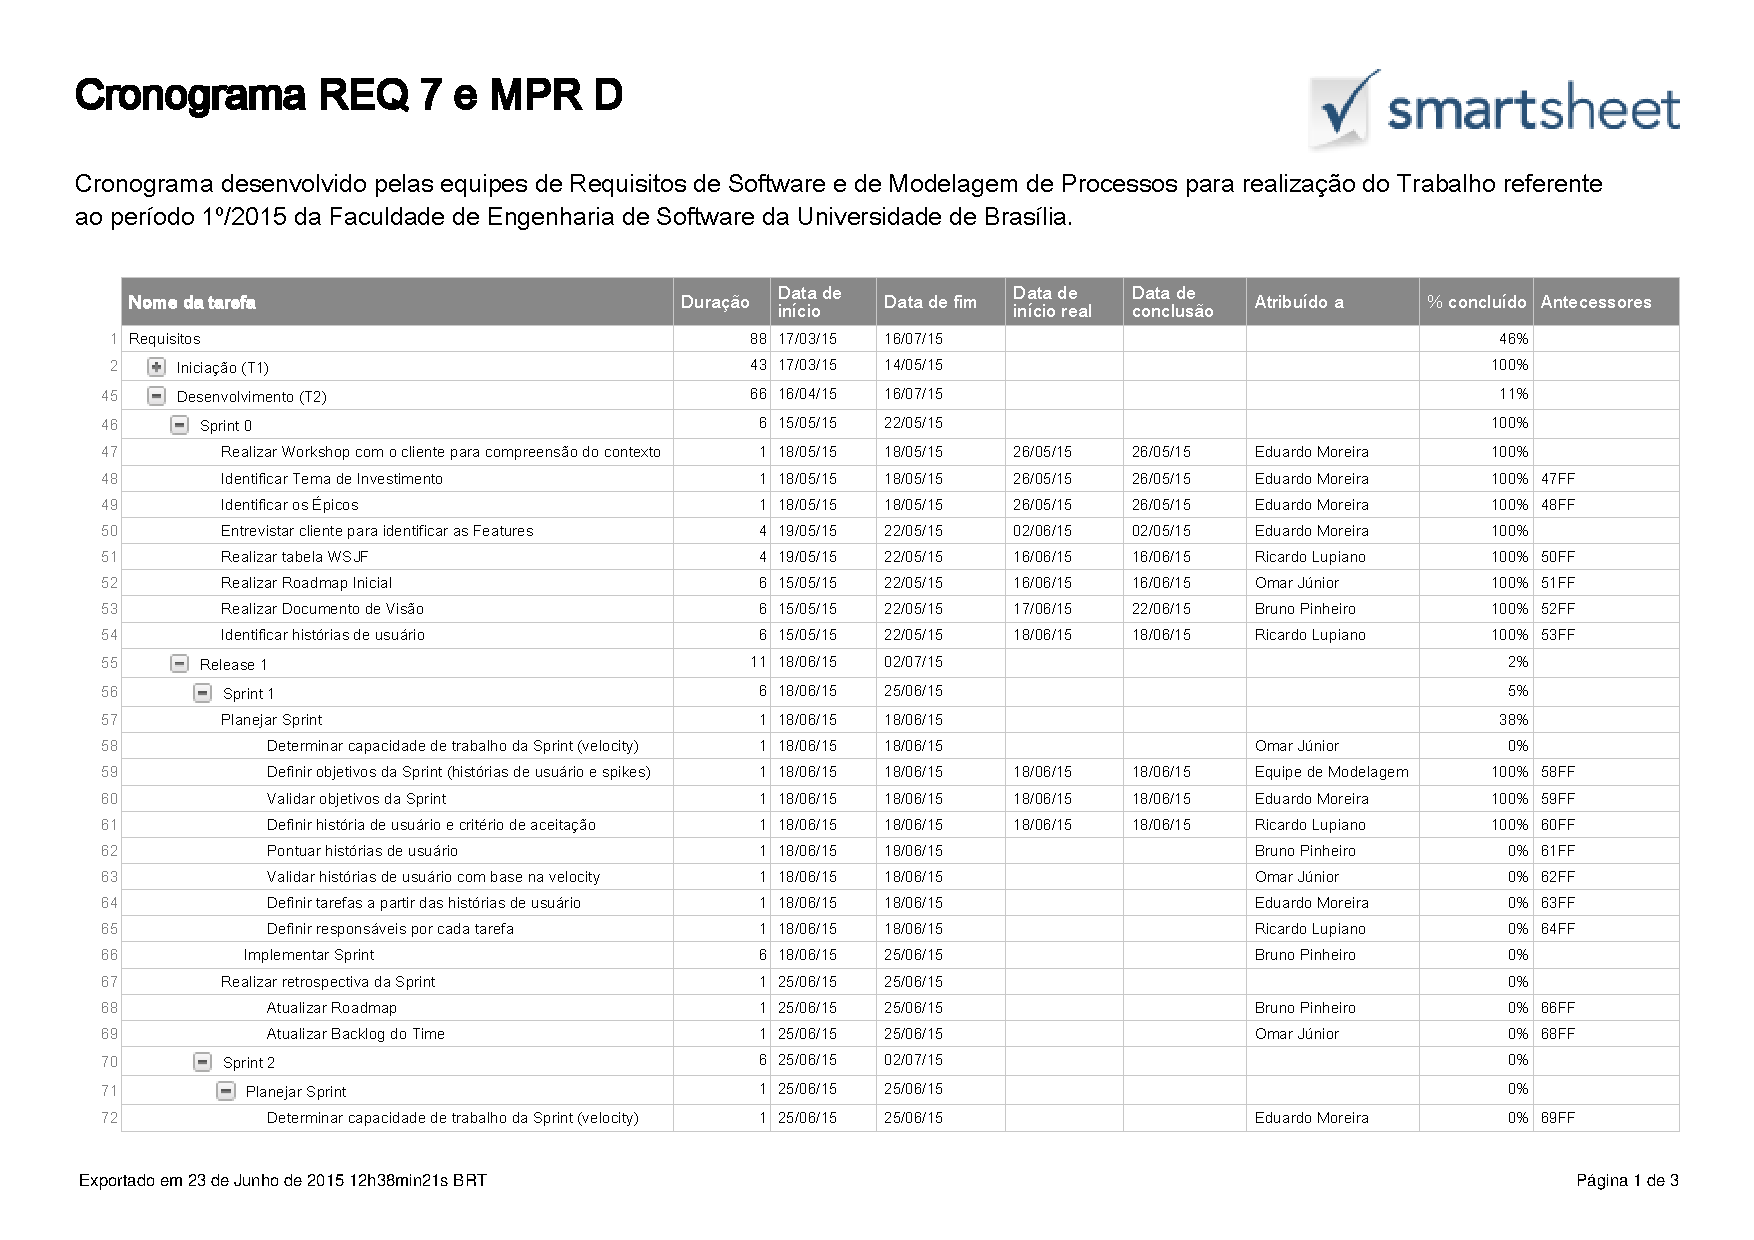
\includepdf[landscape=true, pages=-]{resource/cronograma.pdf}
